\documentclass[10pt,pdf,hyperref={unicode}]{beamer}
\usepackage[utf8]{inputenc}
\usepackage[T1,T2A]{fontenc}
\usepackage[english, russian]{babel}
\usepackage{graphicx}
\usetheme{Rochester}

\title{\huge Практикум }
\author{Серебряков Максим, 311 группа}
\date{Москва 2022}

\begin{document}
\frame[plain]{\titlepage}

\section{Анализ исходных данных}

\begin{frame}
\frametitle{Количество произведенных и сломавшихся мечей для каждой из компании-поставщика за все время}
\begin{figure}[t]
    \centering
    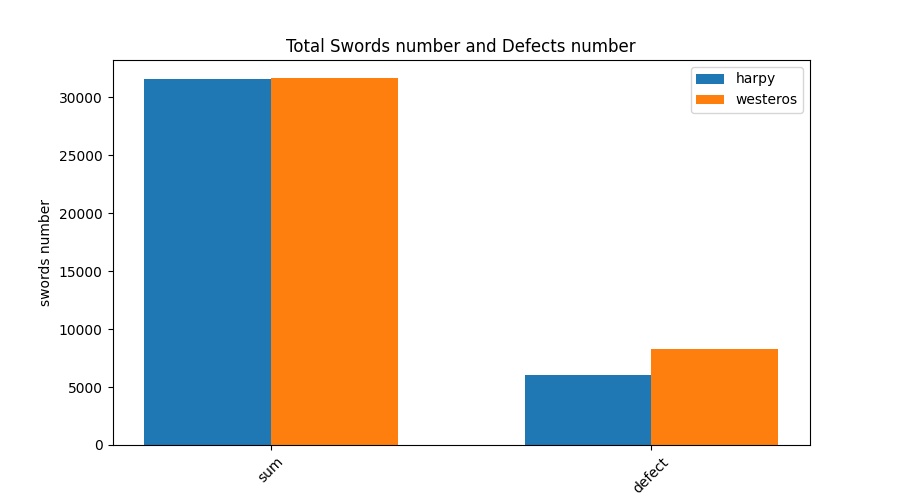
\includegraphics[width=0.9\textwidth]{Figure_1.png}
\end{figure}
Из графика можно заметить, что за время работы количество произведенного оружия из стали компаний практически одинаковое. Но число сломанных мечей из продукции компании Westeros Inс. больше, чем у Harpy \& Co.
\end{frame}

\begin{frame}
\frametitle{Количество произведенных и сломавшихся мечей для каждой из компании-поставщика за все время}

\textbf{Процентное соотношение дефектов к общему числу мечей:} \\
Percentage of defects to total swords number from Harpy: 19.28\% \\
Percentage of defects to total swords number from Westeros: 26.14\%
\end{frame}

\begin{frame}
\frametitle{Среднее число дефектных мечей у одного кузнеца}
\begin{figure}[t]
    \centering
    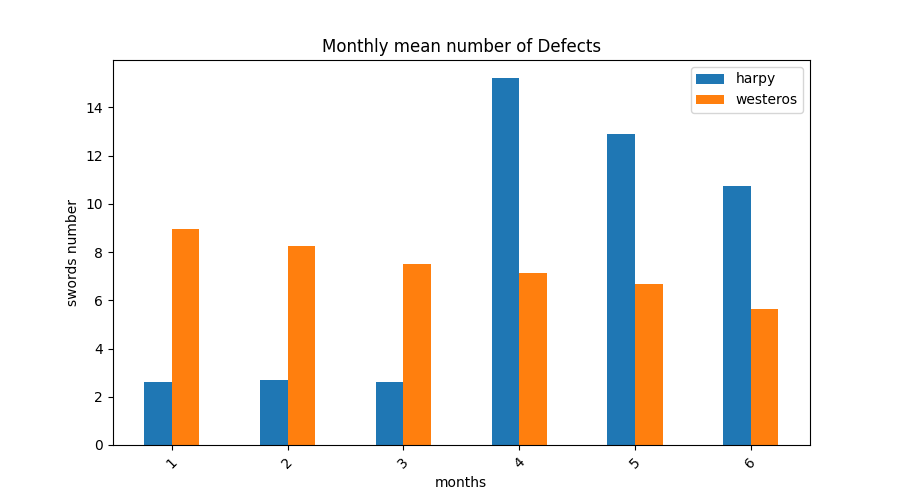
\includegraphics[width=0.9\textwidth]{Figure_2.png}
\end{figure}
Из графика можно заметить, что, в среднем, за первые три месяца мечи из стали Westeros ломаются намного чаще, чем Harpy, но с 4 месяца заметно подрастает количество поломок и у Harpy.
\end{frame}

\begin{frame}
\frametitle{Продолжительность жизни дефектных мечей}
\begin{figure}[t]
    \centering
    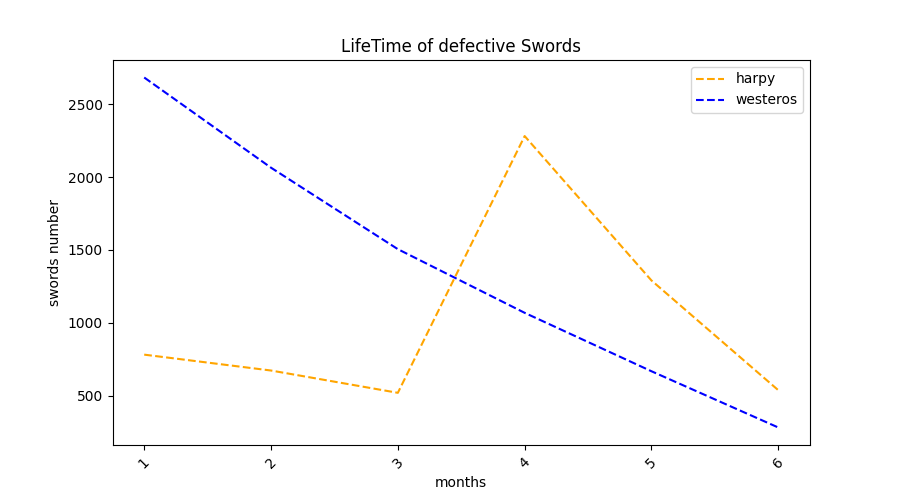
\includegraphics[width=0.9\textwidth]{Figure_3.png}
\end{figure}
Из графика можно понять, что мечей, которые служат меньшее количество времени, больше у Westeros, чем у Harpy, поэтому больше мечей Harpy остаются целыми. 
\end{frame}

\section{Итог}

\begin{frame}
\frametitle{\insertsection}
    \begin{block}{Вывод}
    Исходя из полученных результатов и моих размышлений, стоит заключить договор с компанией Harpy & Co, так как их сталь служит дольше и мечи в первые месяцы не ломаются в таком количестве, как у Westeros Inc. 
    \end{block}
\end{frame}

\end{document}
